\section{Результаты вычислений}
\subsection{Описание экспериментов}
Первый эксперимент: нейронная сеть обучается на первом дикторе с мужским голосом, тестирование производится на каждом дикторе. 

Второй эксперимент: нейронная сеть обучается на всех дикторах с мужским голосом, тестирование производится на каждом дикторе. 

Третий эксперимент: нейронная сеть обучается на всех дикторах, тестирование производится на каждом дикторе.


Было проведено 3 вычислительных эксперимента для каждого из типов.

В процессе тренировки после каждой эпохи тренировочные данные перемешиваются. 15\% тренировочных данных в каждой эпохе - валидационные. В качестве метрики для оценки эффективности была выбрана метрика точности (accuracy), а для валидации - функция потерь категориальной кросс-энтропии (val\_loss). Алгоритм оптимизации - Adam. Максимальное количество эпох - 50. Если значение метрики val\_loss не уменьшается в течение 20 эпох, то обучение останавливается.

Графики обучения для каждого из экспериментов приведены на рисунках \ref{fig:cnn_speaker1_train_graphs}, \ref{fig:cnn_all_male_speakers_train_graphs}, \ref{fig:cnn_all_speakers_train_graphs}.

В конце каждого эксперимента проводится тестирование нейронной сети.
А в случае обучения на all\_speakers помимо тестирования производится построение матрицы ошибок (confusion matrix) для каждого диктора и для каждого из четырех пороговых значений: 0.5, 0.6, 0.7, 0.8. Матрицы представлены на рисунке \ref{fig:cnn_cm_all_speakers}.

Результаты тестирования представлены в таблице \ref{table:test_summary}. Обозначения, которые используются:

all\_speakers = [speaker1, speaker2, speaker3, speaker4, speaker5, speaker6]

all\_male\_speakers = [speaker1, speaker2, speaker3, speaker4, speaker5]

\begin{figure}[H]
  \[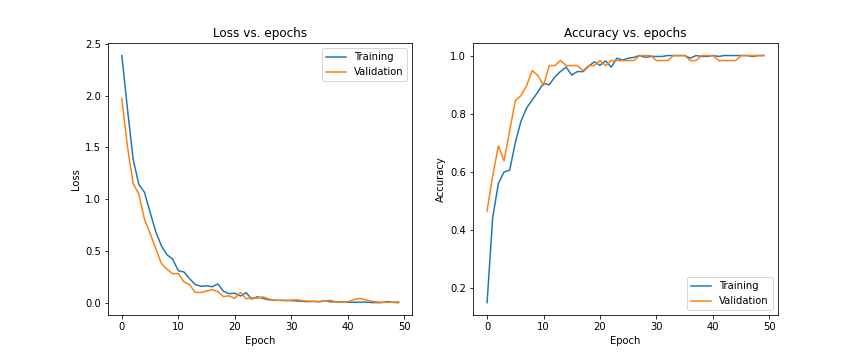
\includegraphics[scale=0.4]{cnn_speaker1_train_graphs.png}\]
  \caption{Графики функции потерь и точности в течение обучения на speaker1}
  \label{fig:cnn_speaker1_train_graphs}
\end{figure}

\begin{figure}[H]
  \[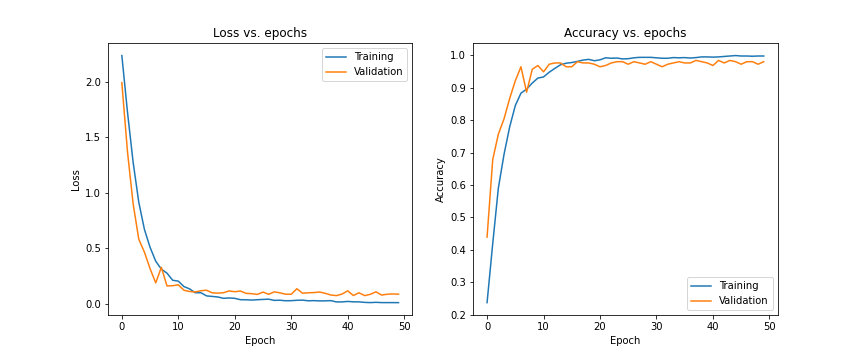
\includegraphics[scale=0.4]{cnn_all_male_speakers_train_graphs.png}\]
  \caption{Графики функции потерь и точности в течение обучения на all\_male\_speakers}
  \label{fig:cnn_all_male_speakers_train_graphs}
\end{figure}

\begin{figure}[H]
  \[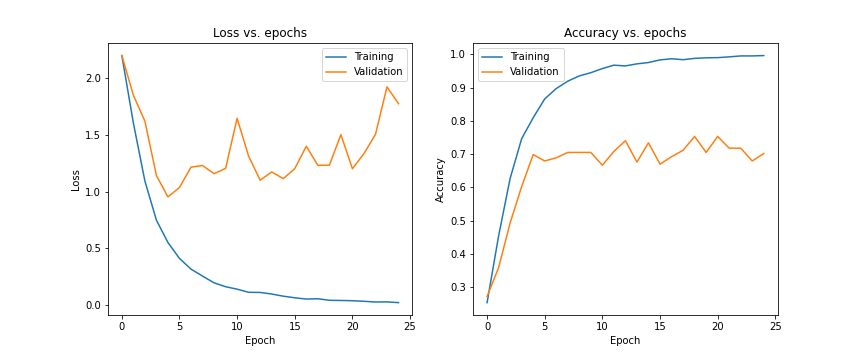
\includegraphics[scale=0.4]{cnn_all_speakers_train_graphs.png}\]
  \caption{Графики функции потерь и точности в течение обучения на all\_speakers}
  \label{fig:cnn_all_speakers_train_graphs}
\end{figure}


\begin{table}[H]
\small
\centering
\csvautotabular[respect underscore=true]{csv/test_summary.csv}
\caption{Результаты вычислений}
\label{table:test_summary}
\end{table}

\begin{figure}[H]
  \[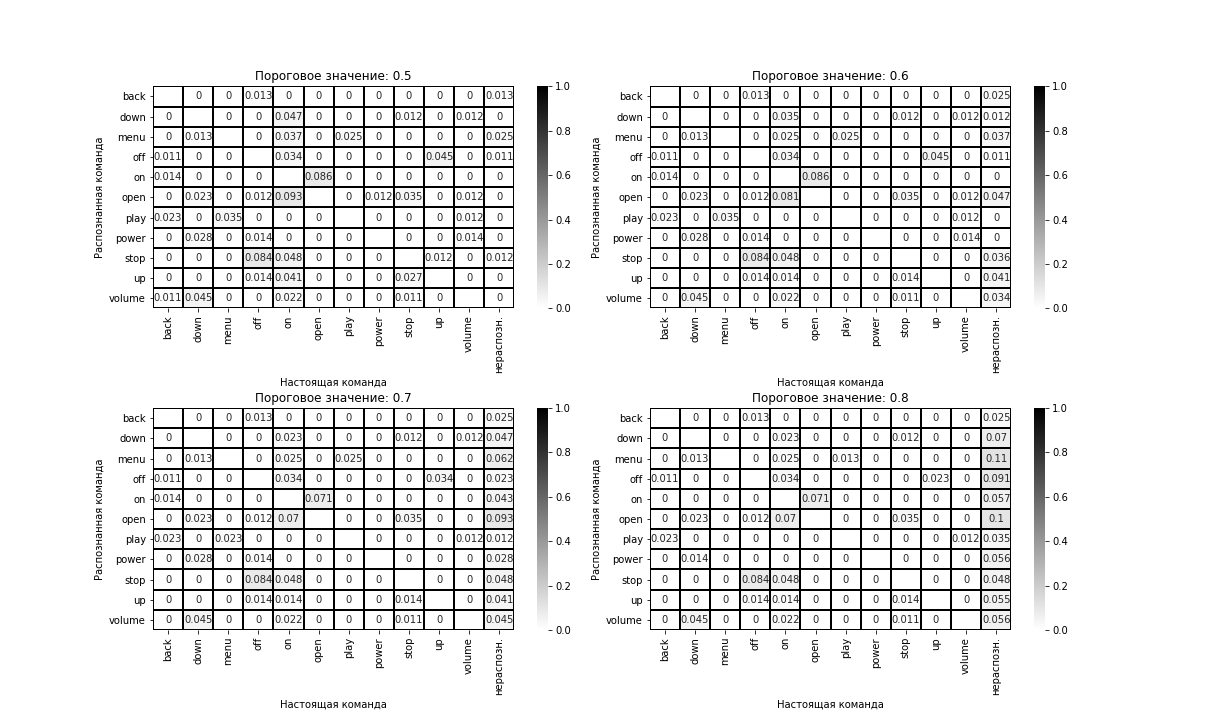
\includegraphics[scale=0.4]{cnn_cm_all_speakers.png}\]
  \caption{Матрицы ошибок для случая обучения на all\_speakers}
  \label{fig:cnn_cm_all_speakers}
\end{figure}
